% !TEX root =../main.tex
\chapter{Posicionamiento mediante marcadores visuales}\label{chp:2}


%%% Figuras %%%%
\def\figFlow{
%TODO: añadir conexión con autopiloto y pequeña descripción interna
\begin{figure}
\includegraphics[width=\textwidth]{posicionamiento_marcadores/tikz/diagrama_flujo}
\caption{A la izquierda: diagrama de flujo del programa que se corre en el ordenador embebido, a la derecha: algunas de las tareas del autopiloto}
\label{fig:flow}
\end{figure}
}

\def\figEjes{
\begin{figure}
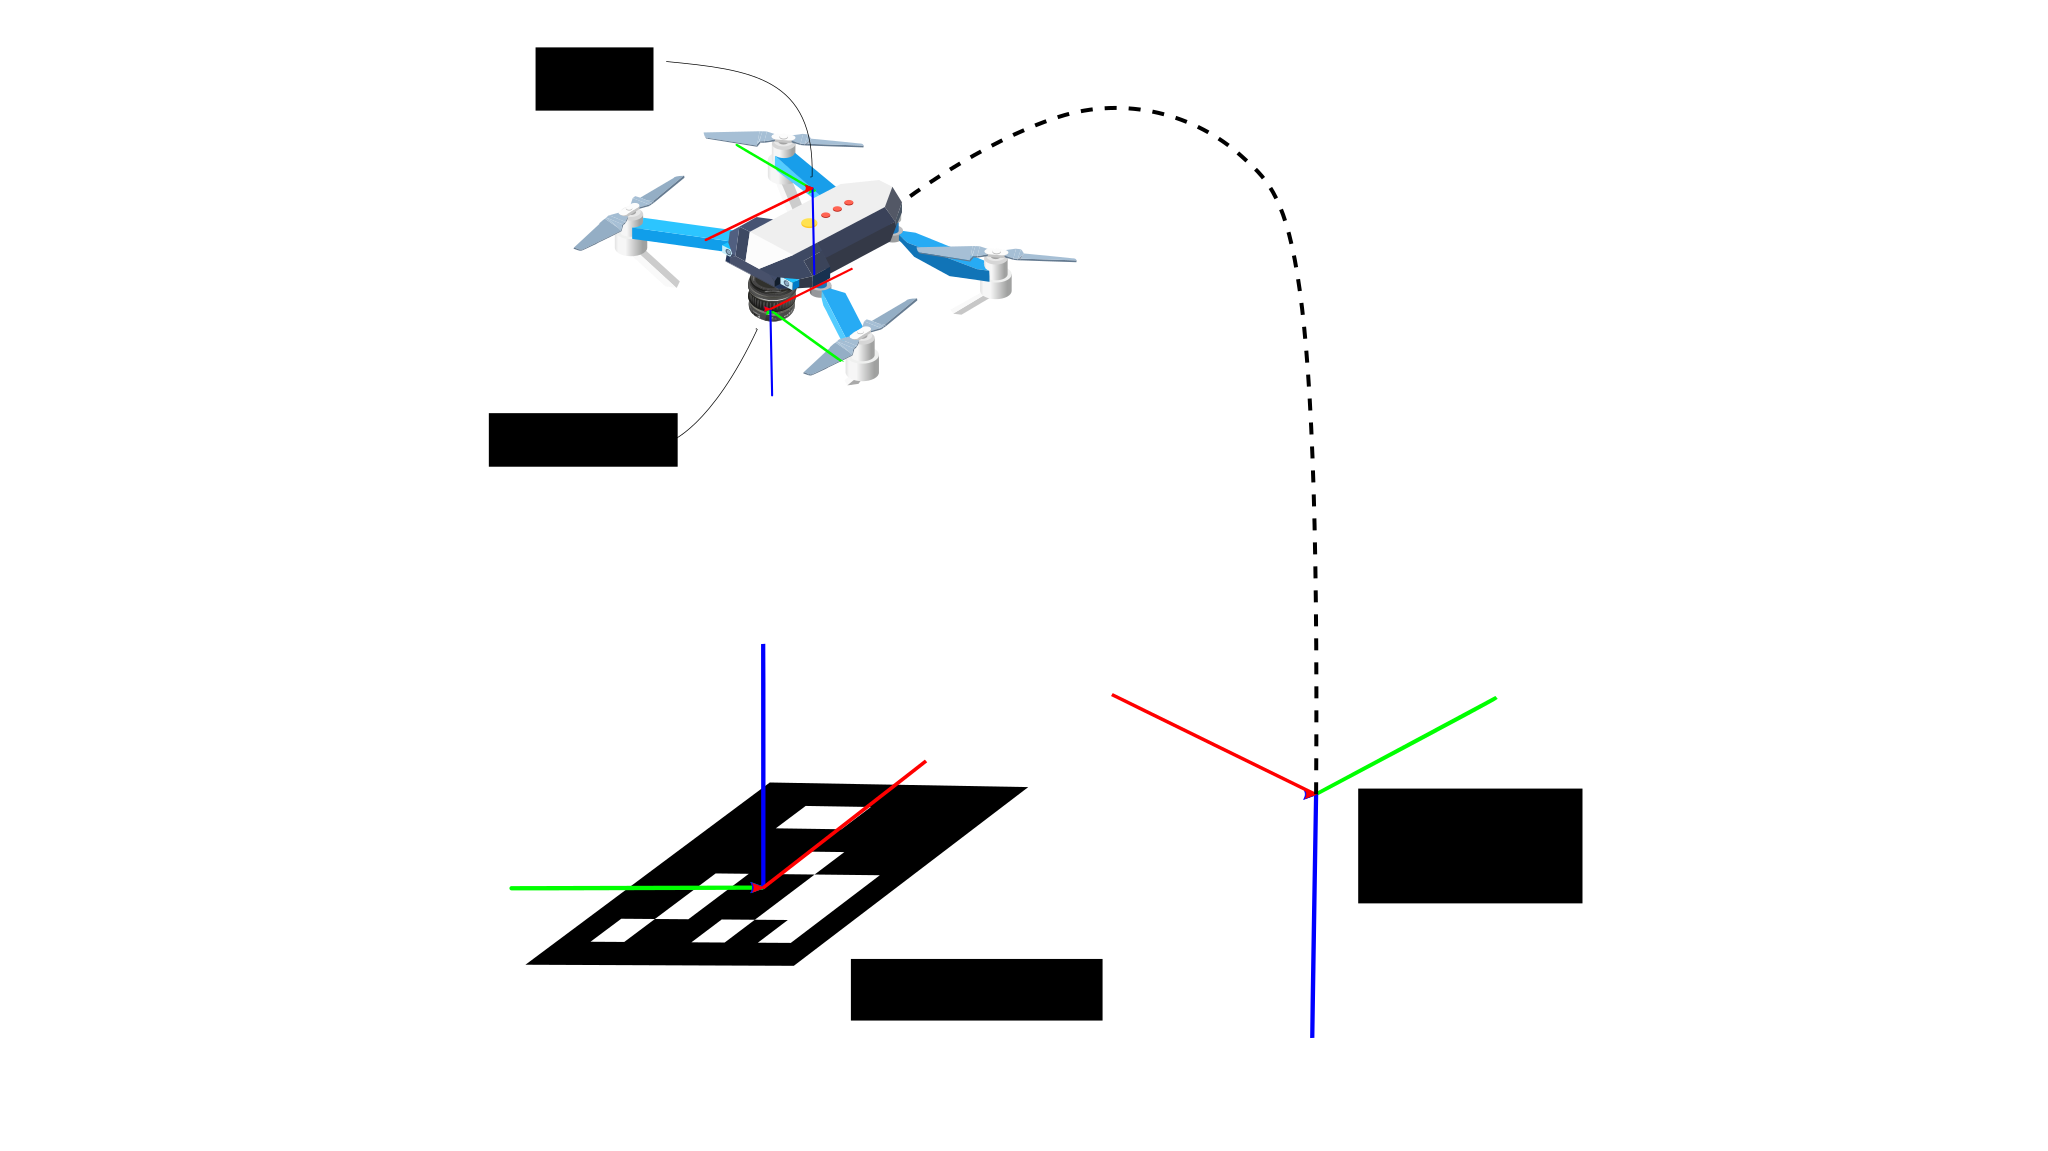
\includegraphics[width=\textwidth]{posicionamiento_marcadores/ejes}
\caption{Sistemas de referencia presentes en el problema}
\label{fig:ejes}
\end{figure}
}

\def\figComp{
\begin{figure}
	\centering
	\begin{subfigure}[t]{\textwidth}
		\centering
		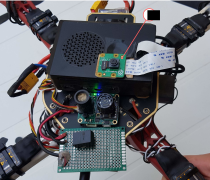
\includegraphics[width=\textwidth]{posicionamiento_marcadores/componentes.pdf}
		\caption{Vista desde arriba}\label{fig:comp1}		
	\end{subfigure}
	\quad
	\begin{subfigure}[t]{\textwidth}
		\centering
		\includegraphics[width=\textwidth]{posicionamiento_marcadores/componentes_abajo.pdf}
		\caption{Vista desde abajo}\label{fig:comp2}		
	\quad
	\end{subfigure}
\caption{Componentes del quadrotor}
\label{fig:comp}
\end{figure}


}


% Más concretamente la precisión que se busca es centimétrica, pensando en coger un objeto metálico de manera autónoma con un imán colgando del UAV

%\lettrine[lraise=-0.1, lines=2, loversize=0.2]{C}{onseguir} con precisión la posición de un vehículo aéreo no tripulado es bastante deseable. En la introducción se comentó aplicaciones como la manipulación de objetos o la navegación cerca de obstáculos. En este cápitulo se explica que para conseguirlo se ha construido un quadrotor con los componentes necesarios para detectar un marcador visual y cómo se ha programado un ordenador embebido en el quadrotor para que procese dicho marcador. 
\lettrine[lraise=0.1, lines=2, loversize=0.1]{C}{onseguir} con precisión la posición de un vehículo aéreo no tripulado es bastante deseable. En la introducción se comentó aplicaciones como la manipulación de objetos o la navegación cerca de obstáculos. En este capítulo se explica que para conseguirlo, se ha construido un quadrotor con los componentes necesarios para detectar un marcador visual. Además, se comenta cómo se ha programado un ordenador embebido para que procese dicho marcador. 

\section{Componentes}
Para elegir los componentes se ha tenido en cuenta que no estén discontinuados, para comprar posibles recambios, la rapidez de llegada ya que todos llegan por paquetería, que estén ampliamente probados, y que en la medida de lo posible estuvieran liberados tanto su software como su hardware. 
\figComp

\begin{enumerate}
\item Cuav V5+. Autopiloto corriendo PX4. Esquemáticos publicados en \href{https://github.com/ArduPilot/Schematics/tree/master/CUAV/V5_Autopilot/V5\%2B}{Github}.
\item \textit{Tattu Funfly 1500mAh}. Batería LiPo de 4 celdas.
\item \textit{DJI 2312E 800KV}. Motor sin escobillas.
\item Hélices de fibra de carbono con un diámetro 9.4 pulgadas y un paso de 5 pulgadas. Según el \href{https://www.dji.com/e305/spec}{fabricante} del motor, con esta hélice se consigue un empuje de 850 gramos alimentado a 14.8 V.
\item \textit{DJI F450}. Chasis de quadrotor de 45 cm de diagonal. 
\item Cama amortiguadora para el autopiloto.
\item Módulo de telemetría \textit{Holybro V3}. Permite una comunicación con la estación de control terrestre.
\item Receptor \textit{X8R}. Recibe hasta 16 canales de la emisora, que este caso es una \textit{Taranis Q X7}. 
\item \textit{SILABS CP2102}. Puente USB-UART. Se conecta entre el puerto USB del ordenador embebido y el puerto UART del autopiloto.
\item CUAV NEO V2. Este incluye GNSS, magnetómetro, botón de armado, luces indicadoras y alarma sonora.

\item Raspberry Pi 4 Model B. 4 GB de RAM. Se encuentra protegida por una carcasa que incorpora un ventilador. 
\item Raspberry Pi Camera Module v2. Campo de visión horizontal de 62 grados, capaz de grabar vídeo con resolución de 1640x1232 a 40fps.
\item \textit{CUAV HV PM (High-Voltage Power Module)}. Regulador de voltaje para alimentar el autopiloto. Además, lee el voltaje y la corriente que suministra la batería. 
\item \textit{Hobbywing XRotor 40A}. Variador de velocidad o ESC. Estos están sobredimensionados ya que fabricante recomienda unos que soporten cómo mínimo una corriente de 20A.
\item \textit{RS PRO K7805-2000R3L}. Reductor de voltaje de 5V y 2A. Este se utilizará para alimentar al ordenador embebido a partir de la batería. Su voltaje permitido de entrada está entre los 8V y los 32V, lo cual es adecuado para una batería LiPo de 4 celdas. 
\item \textit{CUAV PX4FLOW 2.1}. Sensor de flujo óptico. También tiene su \href{https://github.com/PX4/PX4-Flow}{sofware} liberado y el \href{https://github.com/pixhawk/Hardware/tree/master/FLOWv1}{esquemático} de una versión anterior.
\item Extensor de piernas. Estás fueron impresas mediante la empresa \href{https://impresion3dlowcost.es/}{Impresion 3D LowCost} con un modelo tomado de la página \href{https://www.thingiverse.com/thing:915639}{Thingiverse}. Son necesarias ya que el chasis tiene unas patas demasiado cortas y no dejaban espacio para la Raspberry Pi y su cámara. 
\end{enumerate}

%TODO: Tomar foto y enumerar componentes


\section{Programa ejecutado en el ordenador embebido}
De forma resumida, la cámara, que se ha colocado una cámara en la parte inferior del quadrotor y conectada al ordenador embebido, captura imágenes de un marcador que se ha impreso y se ha colocado en el suelo. Este ordenador las procesa y genera una posición estimada del UAV con respecto al marcador, que es enviada al autopiloto a través del puerto serie. El autopiloto la fusiona en su estimador de estados y genera una posición estimada que alimenta al controlador de posición.  El controlador de posición toma esta medida y sigue la referencia. Esta última puede venir o bien del mando o del ordenador embebido el cual le indique una trayectoria.

% generando consignas de aceleración en ejes cuerpo en función de los errores de posición en ejes cuerpo
Nótese que el controlador de posición también se podría haber ubicado en el ordenador embebido, generando consignas de inclinación al autopiloto. 
La desventaja de esto es que se no se utilizan los demás sensores para el posicionamiento.
De la manera que aquí se ha implementado, si en un instante falta la medida de la visión, el autopiloto podría tomar otras como la del acelerómetro, el GPS o el flujo óptico, para fusionarlas en su estimador de estados mientras se espera a que se recupere la medida de la visión.

En la figura \ref{fig:flow} se puede ver el diagrama de flujo del programa que se corre en la Raspberry Pi, cuyos pasos se detallarán a continuación.

% TODO: Poner un trocito de código de cada programa

\figFlow

\begin{enumerate}
\item Inicialización:

	En este paso se espera a detectar el autopiloto y se leen los parámetros de un archivo dedicado a ello.

\item Recoger imagen de la cámara: 

	Este paso podría llegar a ser muy lento si no se escoge una interfaz con la cámara adecuada, por ejemplo USB. En este caso se ha escogido CSI, que lleva la imagen directamente a la GPU y esta la transfiere a la RAM mediante DMA \footnote{Para más información del proceso de captura visitar la excelente documentación de la interfaz Python de la cámara: \url{https://picamera.readthedocs.io/en/release-1.13/fov.html\#division-of-labor}}. Esta tiene la desventaja que el cable es plano y más difícil de torsionar. La ventaja es que la imagen llega a la RAM sin sin consumir tiempo de CPU permitiendo que esta haga en paralelo otras operaciones como el procesamiento de imagen.

\item Detectar marcadores: 

	El objetivo es ubicar los marcadores en la imagen (en concreto sus 4 esquinas) y extraer su identificador.  Este proceso está explicado en \cite{aruco2014}. 
%	- 1. El primer paso es la extración de bordes a partir de la imagen convertida a blanco y negro. 
%	- 2. A partir de la imagen binaria del paso anterior, se extraen los contornos usando en \textit{\_findMarkerContours()} la función de OpenCV  \textit{}
%	- 3. Se realiza una aproximación poligonal y se quedan aquellos que solo estén compuestos por 4 puntos. 

\item Estimación de la posición:

	La estimación de la posición y la orientación se realiza tomando las esquinas de un marcador obtenido en el paso anterior. Este problema se denomina PnP (Perspectiva desde n puntos) y su solución es iterativa. Parte de que, dados unos puntos 3D en el espacio, expresados en un sistema de referencia exterior a la cámara y dada la posición de la cámara con respecto a dicho sistema de referencia, se puede predecir que posición en el plano de la imagen tendrían esos puntos al ser proyectados. Lo que se busca es exactamente lo contrario: la posición de la cámara con respecto a dicho sistema de referencia a partir de la proyección de unos puntos tridimensionales en la imagen. Lamentablemente no se puede invertir las ecuaciones y por tanto no se puede obtener una solución analítica. Para hallar la solución se recurren a algoritmos de optimización que van probando posiciones de la cámara, hacen proyecciones suponiendo esa posición y se compara con las proyecciones reales. A la diferencia de estas dos proyecciones se le denomina \textit{error de reproyección} y es el valor que se trata de minimizar. Para este proyecto este problema no se ha tenido que implementar, solo se ha tenido que llamar a la función \textit{estimatePoseSingleMarkers} de la librería Aruco, que a su vez llama a la función \href{https://docs.opencv.org/4.5.0/d9/d0c/group\_\_calib3d.html\#ga549c2075fac14829ff4a58bc931c033d}{\textit{solvePnP}} de OpenCV.

% No se han utilizado matrices de transformación homogénes porque su inversión no es igual a su traspuesta. Existe un método computacionalmente eficiente pero no es tan intuitivo https://mathematica.stackexchange.com/a/106260

\item Inversión de posición y orientación:
	\figEjes

	Como se ve en la figura \ref{fig:ejes} hay varios sistemas de referencia que entran en juego y hay que tenerlos presentes para transformar desde lo que aporta la estimación de la posición hasta lo que necesita el autopiloto. En el paso anterior, la orientación y posición que se obtiene es la del \textbf{marcador con respecto a la cámara}, es decir se obtiene $R^{C\acute{a}mara \rightarrow Marcador}$ y $p^{C\acute{a}mara \rightarrow Marcador}$. Lo primero que se realiza es buscar la orientación de la cámara con respecto al marcador. Para ello tenemos que invertir la orientación dada, la cual al ser una matriz de rotación, se puede obtener mediante su traspuesta:

	\begin{equation}
	R^{Marcador \rightarrow C\acute{a}mara } = \left(R^{C\acute{a}mara \rightarrow Marcador}\right)^T
	\end{equation}


Dicha matriz se utiliza para expresar la posición del marcador en unos ejes paralelos a los ejes del marcador. 
	\begin{equation}
	p^{C\acute{a}mara' \rightarrow Marcador} = R^{Marcador \rightarrow C\acute{a}mara} \cdot p^{C\acute{a}mara \rightarrow Marcador}
	\end{equation}
Nótese que esta posición sigue teniendo origen en la cámara, solo que ahora está rotado el sistema de referencia en el que se expresa. Lo que se quiere obtener es la posición con respecto al sistema de referencia del marcador, el cual es paralelo al que se está expresando ahora. Siempre que existen dos sistemas de referencia A y B, con la misma orientación pero ubicados en distintos puntos, se debe de negar la posición de A con respecto a B para conseguir la posición de B con respecto a A. Por esta razón la posición que finalmente se le manda al autopiloto es la negada de la obtenida en la última ecuación.   
	\begin{equation}
	p^{Marcador \rightarrow C\acute{a}mara' } = - p^{C\acute{a}mara' \rightarrow Marcador}
	\end{equation}

 En cuanto a la orientación, como se ve en la figura, los ejes de la cámara y los del UAV están rotados 180\textdegree con respecto al eje z. Conociendo esto se obtiene la orientación del marcador visto desde el sistema de referencia del UAV:

	\begin{align}
	R^{UAV\rightarrow C\acute{a}mara}& = \begin{bmatrix} -1 & 0 & 0\\ 0 & -1 & 0 \\ 0 & 0 & 1 \end{bmatrix}\\
	R^{UAV \rightarrow Marcador}& = R^{UAV\rightarrow C\acute{a}mara}\cdot R^{C\acute{a}mara\rightarrow Marcador}
	\end{align}
Es muy importante que la multiplicación se realice en ese orden, ya que la multiplicación de matrices no es conmutativa. De esta manera, la rotación se realiza con respecto al eje z de la cámara, mientras que si se hubiese invertido el orden, es decir se postmultiplica a $R^{C\acute{a}mara\rightarrow Marcador}$, la rotación se hubiese hecho alrededor del eje z del marcador.
	Finalmente, esta última matriz se transpone para tener la orientación del UAV con respecto al marcador.
	\begin{align}
	R^{Marcador \rightarrow UAV}& = \left(R^{UAV \rightarrow Marcador}\right)^T
	\end{align}
	Tras expresar esta rotación en ángulos de euler, ya se podría enviar al autopiloto.
	Estos cálculos están implementados en a partir de la línea \ref{line:invertPose} del archivo \textit{marker\_vision.h} que se ha incluido en el anexo.


	
\item Envio al autopiloto: 

	La orientación y la posición son enviadas al autopiloto a través del protocolo \textit{Mavlink} utilizando la librería \textit{MAVSDK}

\end{enumerate}

Mientras tanto, en el autopiloto, una vez que las recibe, este calcula la rotación entre su orientación expresada en ejes NED y su orientación expresada en el sistema de referencia de la visión, que en este caso es el del marcador. 
\begin{align}
R^{NED \rightarrow Marcador}& =  R^{NED \rightarrow UAV} \cdot  \left(R^{Marcador \rightarrow UAV}\right)^T
\end{align}
Esta matriz se utiliza para transformar la posición que le llega de la visión, expresándola en ejes NED (norte, este y abajo).
\begin{align}
p^{NED' \rightarrow UAV}& = R^{NED \rightarrow Marcador} \cdot p^{Marcador \rightarrow UAV}
\end{align}
Siendo $NED$ el sistema de referencia centrado en la posición que partió el UAV y $NED'$ uno que es paralelo a este último pero centrado en el marcador.
Que tengan está orientación es importante, ya que el EKF en su fase de predicción, utilizando el acelerómetro y la orientación estimada, expresa su posición en ejes NED.
Estos cálculos se pueden ver el código \ref{cod:invPX4} donde se han extraído algunos fragmentos de PX4. 

\begin{codigo}[label=cod:invPX4]{Rotación en PX4 de la posición suministrada por la visión}
En el archivo \href{https://github.com/PX4/PX4-ECL/blob/ec934908900b23ee273d1a9f82364b7b38423200/EKF/ekf\_helper.cpp\#L1460}{\textit{ekf\_helper.cpp}} se calcula la rotación que hay que aplicarle a la posición:
\begin{minted}[firstnumber=1460]{c++}
    const Quatf q_error((_state.quat_nominal * _ev_sample_delayed.quat.inversed()).normalized());
    _R_ev_to_ekf = Dcmf(q_error);
\end{minted}
En el archivo \href{https://github.com/PX4/PX4-ECL/blob/ec934908900b23ee273d1a9f82364b7b38423200/EKF/control.cpp\#L273}{\textit{control.cpp}} se aplica dicha rotación:
\begin{minted}[firstnumber=273]{c++}
    ev_pos_meas = _R_ev_to_ekf * ev_pos_meas;
    ev_pos_var = _R_ev_to_ekf * ev_pos_var * _R_ev_to_ekf.transpose();
\end{minted}
\end{codigo} 

Con estas transformaciones ya se podría fusionar la medida de la visión. Así, se generarán unos estados estimados que serán tomados por los controladores de PX4. Como se explicó en \cite{arias2019control} estos forman una estructura en cascada cuyo controlador de mayor nivel es el de posición. 




\section{Registro de resultados (logging) y análisis} 

\ifthenelse{\entregar = 1}{}{

En este problema hay muchos parámetros que se pueden tocar:
- Número de marcadores
- Tiempo de exposición de la cámara
- Iteraciones máximas de los algoritmos visuales
- Mínima calidad permitida en el reconocimiento de un marcador 

Hay dos maneras de solucionar problemas en ingenieria:
- Planificando y haciendo análisis. Esto es lo ideal ya que cada parámetro o configuración está definida a priori tiene su razón y le pueden respaldar las matemáticas
- Probando y viendo resultados. A veces el entorno real no es completamente predecible, los modelos no funcionan. O simplemente te has equivocado en los cálculos.

Lo ideal es una fusión de ambos. El estudio teórico, sirve para ver que efecto pueden tener los parámetros, también para darles un valor inicial para hacer las pruebas.  

Para verificar el desempeño de la estimación de la posición y orientación, lo ideal sería tener un groundtruth, por ejemplo con GNSS RTK o con un sistema de visión como \textit{OptiTrack}. En este caso no se tiene y lo que nos queda es inspeccionar los resultados de manera visual, que es suficiente para hayar muchos errores de la estimación. Hay que tener en cuenta que se tiene un sistema dinámico y ni la posición ni la velocidad pueden cambiar brúscamente, por lo tanto si al inspeccionar las gráficas temporales de la posición y orientación esto sucede, probablemente se trate de una estimación erronea. Otra forma de verificación es la de ver los ejes del marcador superpuestos en la imagen. Resulta muy fácil de inspeccionar si estos se están moviendo cuando la cámara no cambia de posición.    

% TODO: redactarlo mejor que en lista
Funcionalidades implementadas:
- Archivo de parámetros
- Desactivar la espera de la comunicación del autopiloto
- Tomar las imágenes de un vídeo en lugar de la cámara
- Guardar la posición y orientación estimadas en un archivo. Representación de estas en una gráfica temporal
- Guardar las imágenes de la cámara con los ejes del marcador superpuestos  

% La manera rápida es verificar los parámetros directamente volando y con inspección visual. Así es como se rompe y te gastas dinero
% Problema: el logging puede ser lento, como la escritura de una imagen

A pesar de ser un de ejecución rápida, C++ suele ser más dificil para el desarrollador. En cambio Python es un lenguaje que necesita menos líneas de código para hacer lo mismo, tiene una sintaxis más simple y una cantidad enorme de librerias. Por esta razón, en el programa principal escrito en C++ se han hecho llamadas a sripts de python en el arranque y en la finalización del programa, ya que estos son los momentos en los que es menos crítico el tiempo de ejecución. En concreto, en el arranque se genera una carpeta temporal o se elimina su contenido si ya existía antes. Después, durante la ejecución del bucle principal en el que se estiman las medidas, se pueden guardar diversos resultados dicha carpeta, como la estimación de la posición y la orientación en un archivo CSV o las imágenes capturadas con el sistema de coordenadas del marcador superpuesto.  

}

%\begin{codigo}{Logging en el archivo \textit{main.cpp}}
%\label{cod:invPX4}
%Script de inicio
%\begin{minted}[firstnumber=57]{c++}
%    /* Startup python script for logging */
%    int res=system("python3 ../python_scripts/startup.py");
%    if (res!=0){
%        cout << "El script de inicio ha fallado con código " << res << endl;
%        exit(1);
%    }
%\end{minted}
%Script de finalización
%\begin{minted}[firstnumber=57]{c++}
%    res=system("python3 ../python_scripts/shutdown.py");
%    if (res!=0){
%        cout << "El script de finalización ha fallado con código " << res << endl;
%        exit(1);
%    }
%\end{minted}
%Guardado de la posición y orientación estimada
%\begin{minted}[firstnumber=57]{c++}
%        if (log_file){
%            double seconds = getTickCount()/ getTickFrequency() - seconds_init;
%            myfile << pos[0] << "," << pos[1] << "," << pos[2] << "," << euler_angles[0] << "," << euler_angles[1] << "," << euler_angles[2] << "," << seconds << "\n";
%        }
%\end{minted}
%\end{codigo} 



% Colocar imágenes como ejemplo de problemas detectados. 


\endinput
